% ============================================================
%  paper2.tex -- Framework and results manuscript
%  "Self-Validation Is Not Validation"
%
%  Compiles with pdfLaTeX OR XeLaTeX. No raw Unicode.
%  Overleaf: upload this file plus the figures/ folder, hit Recompile.
%  Local:    pdflatex paper2.tex   (run twice for cross-refs)
%
%  FIGURES: the 5 PDFs this paper needs live in figures/ alongside
%  this file (copied from thesis_assets/figures/ch4/); \graphicspath
%  below points there and all 5 \includegraphics calls are active.
%
%  The expert evaluation sub-study is deliberately EXCLUDED.
%  Placeholders are marked \TODO{...} and render in red.
% ============================================================
\documentclass[11pt,a4paper]{article}

\usepackage[margin=1in]{geometry}
\usepackage{amsmath,amssymb}
\usepackage{booktabs}
\usepackage{longtable}
\usepackage{array}
\usepackage{graphicx}
\usepackage{caption}
\usepackage{xcolor}
\usepackage{microtype}
\usepackage[hidelinks]{hyperref}

\captionsetup{font=small,labelfont=bf,skip=6pt}
\setlength{\parskip}{0.4em}
\graphicspath{{figures/}}

\newcommand{\TODO}[1]{\textcolor{red}{\textbf{[TODO: #1]}}}

\title{\bfseries Self-Validation Is Not Validation:\\
Quantifying and Characterising the Circularity of Counterfactual\\
Root-Cause Analysis in Injection Molding}

\author{%
  Obadah AlQawasema\thanks{Correspondence: \TODO{email}}\ \ and \ \TODO{Supervisor name}\\[0.4em]
  \small Intelligent Systems Master Program, Palestine Polytechnic University, Hebron, Palestine
}
\date{}

\begin{document}
\maketitle

% ------------------------------------------------------------
\begin{abstract}
\noindent
Counterfactual explanation converts a quality classifier into a prescriptive system: when model inputs are settable process parameters, a counterfactual instance reads directly as a corrective recipe. Such systems conventionally establish that a recipe works by querying the model that generated it --- a criterion identical to the search objective, and therefore a measurement of the optimiser rather than of the recommendation. This paper quantifies the consequence on a real manufacturing dataset. We build a three-tier counterfactual root-cause analysis engine --- SHAP-selected parameters with LIME-derived adjustment directions, a nearest-neighbour-anchored fallback, and an escalation tier --- over a random forest champion trained on 1{,}451 injection-molded road-lens cycles described by 13 process parameters. On the held-out test split the champion classifies at 93.81\% accuracy ($n = 291$) and the engine resolves 140 of 147 non-conforming cycles (95.24\%), producing recipes averaging 4.88 adjusted parameters at 0.5161 scaled proximity. An independently trained multilayer-perceptron verifier, of a different family and seed and taking no part in generation, confirms 9 of those 140 --- \textbf{6.43\%}, a gap of 88.81 percentage points. A centroid-ablation baseline that discards SHAP selection and LIME guidance shows the same pattern (10.00\% confirmed; McNemar exact $p = 0.180$), locating the gap in the shared acceptance criterion rather than in the explanation layer. Sweeping that criterion from 0.55 to 0.95 moves resolution from 95.24\% to 4.76\% and confirmation from 6.43\% to 85.71\%; sweeping the search's iteration budget produces the same coupled movement. Mean distance from a counterfactual to the nearest real conforming cycle is 0.829 in a space where each parameter spans two units, indicating the recipes land where the model labels conformance rather than where conformance has been observed. We recommend that prescriptive quality systems report independent verification alongside self-measured resolution and state their position on this trade-off explicitly.
\end{abstract}

\noindent\textbf{Keywords:} counterfactual explanation; root cause analysis; injection molding; explainable AI; model validation; prescriptive analytics; random forest; SHAP

\vspace{1em}\hrule\vspace{1em}

% ------------------------------------------------------------
\section{Introduction}

Predicting injection molding part quality from machine-native process parameters is established: reported accuracies on public benchmark data exceed 93\%~\cite{polenta2022}. The open question is what to do with a prediction, and counterfactual explanation supplies an unusually direct answer. Because the input features are quantities an operator sets, a counterfactual instance is not a description but an instruction.

That directness carries an evidential burden. A counterfactual is conventionally deemed \emph{valid} when the model assigns it to the desired class --- but it was generated by searching that model's decision surface until the model did so. The criterion of judgement and the objective of construction are the same object. A procedure optimised to reach a point where $P(\text{conforming}) \geq \theta$, and evaluated by checking whether $P(\text{conforming}) \geq \theta$, cannot fail except through search failure. The reported validity rate measures the competence of the optimiser~\cite{laugel2019,keane2021}.

This would be a harmless tautology if trained models faithfully represented their processes. They do not, in documented ways. Laugel et al.\ show that post-hoc counterfactuals can be \emph{unjustified} --- continuously connected to the model's favourable region but not to the data's~\cite{laugel2019}. Rudin argues that post-hoc explanations of black-box models mislead precisely where it matters~\cite{rudin2019}. Slack et al.\ establish that agreement between a model and its explainer is not evidence of correctness~\cite{slack2020}. Surveys of evaluation practice find one XAI paper in three evaluating exclusively on anecdotal evidence~\cite{nauta2023}, and only 21\% of published counterfactual methods user-tested at all~\cite{keane2021}.

What the literature does not contain is a \textbf{measurement}. The discrepancy between what a counterfactual RCA engine reports about itself and what an independent check confirms has never been quantified in an industrial process-control setting, across a full evaluation population rather than on selected illustrative cases. Nor is it known whether such a discrepancy is a property of one search algorithm or of the method class, or whether it is fixed or tunable.

This paper supplies those measurements. Our contributions:

\begin{enumerate}
\item \textbf{A quantification of the circularity gap.} On held-out data, a counterfactual RCA engine reports 95.24\% resolution while an independent verifier confirms 6.43\% of those resolutions --- a gap of 88.81 percentage points, measured across the entire non-conforming test population.
\item \textbf{Evidence that the gap belongs to the method class.} A centroid-ablation baseline sharing only the acceptance criterion reproduces the pattern, with the difference statistically indistinguishable from chance under a paired exact test.
\item \textbf{A characterisation of the gap as a tunable operating characteristic.} Two structurally independent hyperparameters --- the acceptance threshold and the search's iteration budget --- move resolution and confirmation in coupled opposite directions, converting a single unfavourable figure into a design parameter with a measurable cost curve.
\item \textbf{A hybrid SHAP-plus-LIME explanation layer} in which SHAP selects which parameters to adjust and LIME determines direction, yielding deterministic feature selection via exact TreeSHAP and attributions corroborated by two model-free importance methods (Spearman $r = 0.659$ and $0.604$, all three ranking the same parameter first).
\end{enumerate}

% ------------------------------------------------------------
\section{Related Work}

\textbf{Quality prediction in injection molding.} Ribeiro established that learned models detect molding faults at rates exceeding statistical process control~\cite{ribeiroB2005}. Polenta et al.\ compared six classifiers on 1{,}451 road-lens cycles, reporting random forest best at 95.04\% $\pm$ 1.26\% under stratified five-fold cross-validation, and released both dataset and code~\cite{polenta2022} --- the reason we adopt their data here. P\'{a}rizs et al.~\cite{parizs2022} and Ogorodnyk et al.~\cite{ogorodnyk2019} report comparable results on related formulations.

\textbf{Explainability in manufacturing.} Feature attribution dominates, principally SHAP~\cite{lundberg2017} and LIME~\cite{ribeiro2016}. M\"{u}ller et al.\ pair a neural classifier with symbolic rules for interactive industrial quality control~\cite{muller2022}. Explainability remains thin within injection molding specifically.

\textbf{Counterfactual explanation and its critiques.} Since Wachter et al.~\cite{wachter2018}, extensions have addressed diversity~\cite{mothilal2020}, feasibility~\cite{poyiadzi2020}, prototype guidance~\cite{vanlooveren2021} and actionability~\cite{ustun2019}, surveyed by Verma et al.~\cite{verma2024} and Guidotti~\cite{guidotti2024}. Karimi et al.\ separate explanation from recourse, arguing that recommending an action requires causal assumptions a predictive model does not supply~\cite{karimi2021}. The critical strand~\cite{laugel2019,alvarezmelis2018,slack2020,krishna2022,adebayo2018} establishes that model endorsement is weak evidence. Doshi-Velez and Kim's hierarchy~\cite{doshivelez2017} places self-reported validity at the least demanding level available.

\textbf{Our position relative to this work.} The conceptual argument is established. Our contribution is empirical: a measurement of the gap in an industrial setting, a test of whether it generalises across search strategies, and a characterisation of how it varies with the operating point.

% ------------------------------------------------------------
\section{Materials and Methods}

\subsection{Dataset and conformance definition}

We use the dataset released by Polenta et al.~\cite{polenta2022}: 1{,}451 production cycles from the manufacture of plastic road lenses, each described by 13 process parameters recorded by the machine controller and labelled into four quality classes --- \emph{Waste}, \emph{Acceptable}, \emph{Target}, \emph{Inefficient}.

The labels encode two distinct notions. \emph{Waste} denotes parts failing the photometric conformance standard. \emph{Inefficient} denotes parts that conform but were produced under settings consuming unnecessary energy or cycle time. \textbf{Conforming is defined throughout as \{\emph{Acceptable}, \emph{Target}\}}, with \{\emph{Waste}, \emph{Inefficient}\} treated as non-conforming for root-cause analysis. The grouping is applied consistently and is stated explicitly because \emph{Inefficient} parts are physically saleable; the RCA task for them is process-economic rather than quality-remedial.

\subsection{Preprocessing and split discipline}

Features were scaled to $[-1, 1]$ by a min--max transform fitted on the training partition only. The dataset was split 60/20/20 into training ($n = 870$), validation, and held-out test ($n = 291$) partitions with stratification on the quality label and a fixed seed. The test split contains 74 \emph{Waste}, 82 \emph{Acceptable}, 62 \emph{Target} and 73 \emph{Inefficient} cycles, giving \textbf{147 non-conforming cycles}.

\textbf{Test-split figures are reported as the headline throughout, and validation figures appear only as comparison --- including, and especially, where the test figure is the less flattering of the two.} The validation split participated in champion selection and is therefore not a clean estimate~\cite{cawley2010}.

\subsection{Champion classifier and hyperparameter provenance}

The champion is a random forest~\cite{breiman2001} with \texttt{n\_estimators = 151}, \texttt{max\_depth = 79}, \texttt{criterion = 'entropy'}.

\textbf{These values were not tuned in this work.} They are adopted from Table 5 of Polenta et al.~\cite{polenta2022}. Five deviations from the source configuration were required by the implementation and are documented in Table~\ref{tab:hyper}; they arise from \texttt{scikit-learn}~\cite{pedregosa2011} not implementing gain ratio, from the substitution of \texttt{RandomForestClassifier} for extremely randomised trees~\cite{geurts2006} to preserve TreeSHAP compatibility, and from the consequent change to the features-per-split rule. \texttt{max\_depth} carries a further, distinct deviation: the source's Table 5 reports \texttt{max\_depth = 79} against its gain-ratio configuration and \texttt{max\_depth = 140} against its information-gain configuration, and this work pairs the \texttt{'entropy'} (information-gain) criterion with the \emph{gain-ratio} row's depth value, so the two adopted parameters originate from different rows of the source table. The discrepancy is immaterial in practice: the configured \texttt{max\_depth = 79} is not a binding constraint, since realised maximum depth across the 151 estimators is 20, well below either source value.

\begin{table}[htbp]
\centering
\caption{Hyperparameter provenance against Polenta et al.~\cite{polenta2022}, Table 5.}
\label{tab:hyper}
\small
\begin{tabular}{@{}p{0.22\linewidth}p{0.22\linewidth}p{0.22\linewidth}p{0.26\linewidth}@{}}
\toprule
\textbf{Aspect} & \textbf{Reference} & \textbf{This work} & \textbf{Classification / reason} \\
\midrule
Split criterion & Gain ratio & Entropy & Deviation: not implemented in \texttt{scikit-learn} \\
Ensemble type & Extremely randomised trees & \texttt{RandomForestClassifier} & Deviation: TreeSHAP compatibility \\
Features per split & $\lfloor \log(m) + 1 \rfloor$ & \texttt{'sqrt'} (library default) & Equivalent at $m = 13$: both give 3 \\
Maximum depth & 79 (gain ratio row) / 140 (information gain row) & 79 & Deviation: mixed-row provenance \\
Number of trees & 151 & 151 & Identical \\
\bottomrule
\end{tabular}
\end{table}

Our results are consequently \textbf{not a replication} of~\cite{polenta2022} and should not be read as one.

\subsection{Explanation layer}

Global and local attributions are computed with SHAP TreeExplainer~\cite{lundberg2017}, which yields exact Shapley values for tree ensembles in polynomial time. Local linear surrogates are computed with LIME~\cite{ribeiro2016}.

The two are given a defined division of labour: \textbf{SHAP selects which parameters to adjust; LIME determines the direction of adjustment.} This uses each method for the quantity it estimates more reliably --- exact TreeSHAP gives deterministic feature selection, while LIME's signed local coefficients give an adjustment direction that a magnitude-only attribution does not.

\subsection{Three-tier counterfactual engine}

Define the acceptance score $s(\mathbf{x}) = P(\emph{Acceptable} \mid \mathbf{x}) + P(\emph{Target} \mid \mathbf{x})$. A candidate $\mathbf{x}'$ is accepted when $s(\mathbf{x}') \geq \theta$, default $\theta = 0.55$. Search proceeds in scaled space with step 0.02 and an iteration budget of 150, \textbf{clipping every parameter to its observed training range at every iteration}, so that every recommendation lies within the range of values the machine has actually been operated at by construction rather than by post-hoc filtering.

\begin{itemize}
\item \textbf{Tier 0 --- already acceptable.} If $s(\mathbf{x}) \geq \theta$ for the original cycle, no correction is attempted.
\item \textbf{Tier 1 --- SHAP-selected, LIME-directed.} The five parameters with largest local SHAP magnitude are selected; LIME coefficients set each adjustment's sign; parameters move iteratively until acceptance or budget exhaustion.
\item \textbf{Tier 2 --- nearest-neighbour anchored.} On Tier 1 failure, the 15 nearest conforming training cycles are located and the seven highest-magnitude parameters move toward their centroid.
\item \textbf{Tier 3 --- escalation.} On Tier 2 failure the case is reported as structurally uncorrectable within feasible bounds. No recommendation is issued.
\end{itemize}

\textbf{On the cascade's activation.} At $\theta = 0.55$ the cascade does not cascade: all 140 resolved test cases are Tier 1, with zero Tier 2 and zero Tier 3. Tiers 2 and 3 activate only under stricter acceptance criteria --- at $\theta = 0.75$ they take 21 and 33 cases. The tiered architecture is therefore \textbf{a specified fallback at the default operating point rather than an active operating envelope}, and is a precondition for operating anywhere on the high-confirmation region of the trade-off characterised in Section~\ref{sec:sweep}. We state this rather than present the cascade as continuously active.

\subsection{Independent verifier}

Every accepted counterfactual is submitted to a verifier of a different model family: a multilayer perceptron, hidden layers $(100, 50)$, ReLU, Adam, early stopping with patience 20, seed 7. It confirms a counterfactual when it also assigns it to the conforming set.

\textbf{Leakage guarantees.} The verifier, the Tier 2 conforming-neighbour pool, and the ablation centroid derive exclusively from the training partition. Validation and test splits are evaluation targets only and enter no fitting step.

\textbf{What confirmation establishes.} That a counterfactual satisfies a model of a different family, different seed, and no involvement in its generation. \textbf{It does not establish that the recommendation would work on a machine.} Both models are trained on the same data and share whatever biases that data carries; agreement bounds the risk of a model-specific artefact but cannot exclude a shared one.

\textbf{On the verifier's competence.} The MLP family achieved 0.9218 cross-validation mean accuracy and 0.8931 validation accuracy as a standalone candidate. A model classifying real cycles at roughly 90\% is not failing to recognise conforming parameter vectors in general.

\subsection{Centroid-ablation baseline}

To test whether the finding depends on the explanation-guided search, we compare against an ablation that removes it: all parameters move simultaneously toward the centroid of conforming training cycles, with no SHAP selection and no LIME direction. \textbf{Acceptance criterion, step size, bounds, iteration budget, champion model and verifier are held identical.} Matching the acceptance criterion is a design requirement --- otherwise resolution differences would reflect the threshold rather than the ablated components.

\subsection{Deployment context}

The framework is deployed as a multi-page application incorporating ISO 9001 process-capability monitoring, SQLite traceability, PSI and Page--Hinkley drift detection~\cite{page1954}, and operator notification. All experiments ran on CPU with no GPU acceleration at any stage. At the default configuration, 147 non-conforming cycles are analysed in approximately 71~s --- \textbf{0.48~s per cycle} including SHAP attribution, LIME explanation, iterative search and verification --- comfortably within an injection molding cycle time. Full sweeps required 2{,}873~s (test) and 1{,}662~s (validation). \TODO{Insert CPU model, core count, RAM, OS.}

\subsection{Metrics and statistics}

Per non-conforming cycle we record \textbf{resolution} (an accepted counterfactual was produced), \textbf{verifier confirmation}, \textbf{proximity} ($L_2$ from original to counterfactual in scaled space), \textbf{sparsity} (parameters with $|\Delta| > 10^{-4}$), and \textbf{nearest-neighbour distance} ($L_2$ to the nearest conforming training cycle) --- the out-of-distribution measure Keane et al.\ recommend reporting alongside proximity and sparsity~\cite{keane2021}, operationalising the connectedness criterion of Laugel et al.~\cite{laugel2019}.

\textbf{Two denominator conventions must be stated.} Confirmation rate is confirmed cases divided by \textbf{resolved} cases, not by all non-conforming cases: the quantity of interest is the reliability of the recommendations actually issued, and cases the engine declines to answer are not recommendations. Resolution rate, over all non-conforming cases, carries the complementary information.

\textbf{The paired test operates on the raw per-sample verifier flag}, not the resolved-only subset. A Tier 3 escalation carries a negative flag; a Tier 0 already-conforming cycle carries a \emph{positive} flag, because the engine returns a confirmed status for a cycle it declines to modify. Tier 0 cases therefore sit in the concordant cell for both methods and, since McNemar conditions only on discordant pairs, have no effect on the statistic. \textbf{The aggregate rates and the contingency table consequently use different denominators, and both are reported so the difference is visible rather than latent.} Nearest-neighbour distance is structurally biased toward centroid-seeking methods; this is stated in advance and again where results are reported.

McNemar's exact two-sided test~\cite{mcnemar1947} is applied to paired per-sample confirmation outcomes.

% ------------------------------------------------------------
\section{Results}

\subsection{Classifier performance}

Six algorithms were trained on the training split ($n = 870$) and compared by stratified five-fold cross-validation within it, ranked by CV mean in Table~\ref{tab:algcomp}.

\begin{table}[htbp]
\centering
\caption{Six-algorithm comparison, training split, ranked by five-fold CV mean accuracy.}
\label{tab:algcomp}
\small
\begin{tabular}{@{}lcccc@{}}
\toprule
\textbf{Algorithm} & \textbf{CV mean} & \textbf{CV std} & \textbf{Val. accuracy} & \textbf{Val. F1 (weighted)} \\
\midrule
Random Forest          & 0.9471 & 0.0190 & 0.9310 & 0.9306 \\
XGBoost                 & 0.9425 & 0.0202 & 0.9414 & 0.9412 \\
Gradient Boosting       & 0.9379 & 0.0168 & 0.9310 & 0.9307 \\
Multilayer Perceptron   & 0.9218 & 0.0240 & 0.8931 & 0.8924 \\
Decision Tree           & 0.9023 & 0.0170 & 0.8966 & 0.8958 \\
k-Nearest Neighbours    & 0.8839 & 0.0043 & 0.8828 & 0.8814 \\
\bottomrule
\end{tabular}
\end{table}

The top three are closely spaced --- Random Forest, XGBoost and Gradient Boosting span 0.9379 to 0.9471, a range smaller than the cross-validation standard deviation of any of the three --- and the two criteria disagree: XGBoost attains the highest single-split validation accuracy while Random Forest attains the highest cross-validation mean. Selection proceeded on CV mean, and Random Forest is the champion; on the validation split alone the gap is three samples out of 290, a difference at the resolution of sampling noise.

The champion achieves \textbf{93.81\% accuracy} on the held-out test split ($n = 291$), weighted F1 0.9381, macro F1 0.9369, non-conformance precision 0.9329 and recall 0.9456.

\begin{table}[htbp]
\centering
\caption{Per-class performance on the held-out test split ($n = 291$).}
\label{tab:perclass}
\small
\begin{tabular}{@{}lccc@{}}
\toprule
\textbf{Class} & \textbf{Precision} & \textbf{Recall} & \textbf{Support} \\
\midrule
Waste       & 0.9459 & 0.9459 & 74 \\
Acceptable  & 0.9512 & 0.9512 & 82 \\
Target      & 0.9333 & 0.9032 & 62 \\
Inefficient & 0.9200 & 0.9452 & 73 \\
\bottomrule
\end{tabular}
\end{table}

Errors occur exclusively within two adjacent class pairs --- \emph{Waste}/\emph{Acceptable} (4 each way) and \emph{Target}/\emph{Inefficient} (6 and 4) --- with no confusion between the pairs. The consequential error, non-conforming parts classified as conforming, occurs in 4 of 74 \emph{Waste} cycles.

\textbf{Comparison with the reference study.} Polenta et al.\ report 95.04\% $\pm$ 1.26\%~\cite{polenta2022}. Ours is lower, and the protocols differ: theirs is a mean over test folds of stratified five-fold cross-validation across all 1{,}451 samples; ours is a single held-out split of 291. The 1.2-point difference falls within one standard deviation of their fold-to-fold spread, and five hyperparameter deviations separate the configurations. The figures should be read as broadly consistent rather than as a successful or failed replication.

\begin{figure}[htbp]\centering
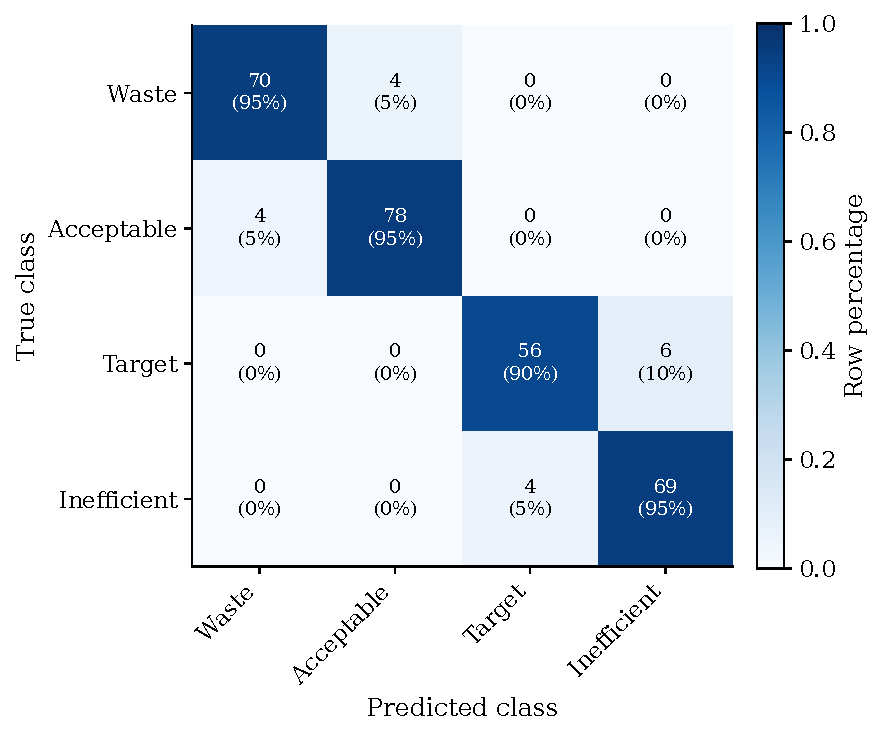
\includegraphics[width=0.7\linewidth]{fig_ch4_confusion_matrix_test.pdf}
\caption{Confusion matrix, held-out test split, counts and row percentages.}
\label{fig:cm}\end{figure}

\subsection{Explanation layer}

The SHAP global ranking was compared against two model-free filter rankings reported in~\cite{polenta2022}. Spearman rank correlation is \textbf{0.659} against Relief and \textbf{0.604} against ANOVA --- moderate positive agreement --- with \textbf{cycle time ranked first by all three methods}.

Moderate rather than strong agreement is the expected result: the filters assess marginal discriminative power model-free, while SHAP measures contribution to a specific fitted model including through interactions. Convergence on the same top parameter across model-free and model-dependent methods is a meaningful corroboration.

\begin{figure}[htbp]\centering
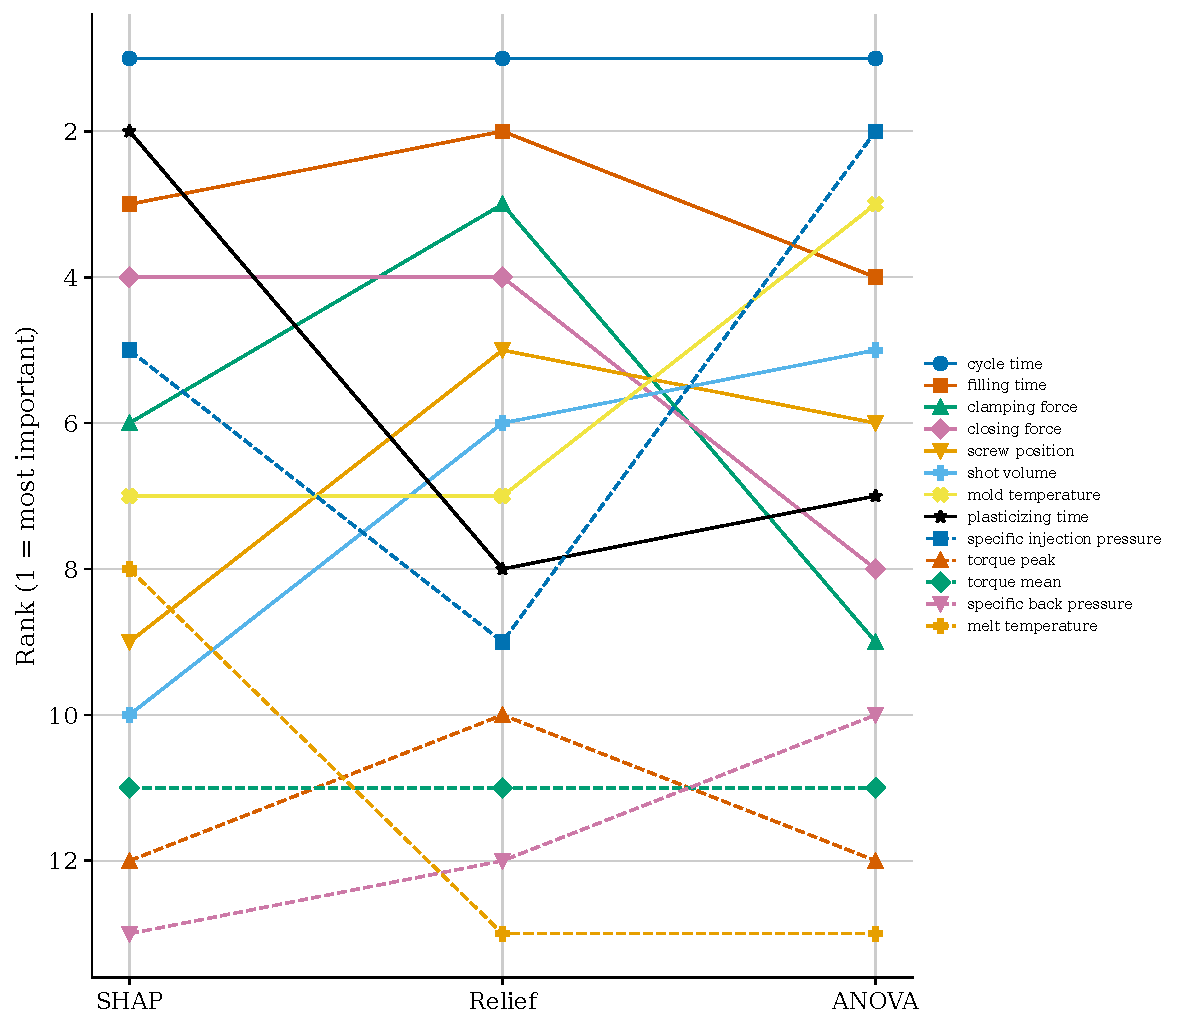
\includegraphics[width=0.8\linewidth]{fig_ch4_importance_method_comparison.pdf}
\caption{Rank comparison of the 13 process parameters across SHAP, Relief and ANOVA.}
\label{fig:ranks}\end{figure}

\subsection{Counterfactual resolution}

The engine resolved \textbf{140 of 147} non-conforming test cycles --- \textbf{95.24\%} --- with mean sparsity 4.88 parameters and mean proximity 0.5161 in scaled units. Every recommendation lies within the machine's observed operating range by construction.

The seven unresolved cases are \textbf{Tier 0 short-circuits} --- cycles the champion already regards as conforming --- not search failures. The test split contains \textbf{zero Tier 3 escalations} at the default configuration. Read as search success the 95.24\% understates (the search succeeded on 140 of the 140 cycles it attempted); read as population coverage it is correct.

A worked case (test index 8) moved an 83.66\% \emph{Waste} cycle to 62.93\% \emph{Target} through adjustments including a 0.46\% change in closing force --- filling faster while plasticizing longer and holding the mold marginally cooler, a recognisable process intervention rather than an arbitrary vector, with near-zero cycle-time change (Table~\ref{tab:worked}). A contrasting case (test index 5) reached 58.01\% conforming confidence with a comparably small and comparably coherent recipe and was \textbf{not} confirmed by the verifier. Nothing on the face of either recipe distinguishes them. That indistinguishability is the subject of the next section.

\begin{table}[htbp]
\centering
\caption{Worked counterfactual case, test index 8, in engineering units (Tier 1, five SHAP-selected parameters).}
\label{tab:worked}
\small
\begin{tabular}{@{}lcccc@{}}
\toprule
\textbf{Parameter} & \textbf{Original} & \textbf{Suggested} & \textbf{$\Delta$} & \textbf{Direction} \\
\midrule
SKx --- Closing force (N)         & 908.6  & 904.424 & $-$4.176  & $\downarrow$ \\
time\_to\_fill (s)                 & 6.968  & 6.5562  & $-$0.4118 & $\downarrow$ \\
Mold temperature ($^\circ$C)      & 81.402 & 81.139  & $-$0.263  & $\downarrow$ \\
ZDx --- Plasticizing time (s)      & 4.08   & 4.3032  & $+$0.2232 & $\uparrow$ \\
ZUx --- Cycle time (s)             & 74.82  & 74.9008 & $+$0.0808 & $\uparrow$ \\
\bottomrule
\end{tabular}
\end{table}

\subsection{The circularity finding}\label{sec:circ}

\begin{table}[htbp]
\centering
\caption{Self-reported resolution against independently confirmed resolution, default configuration.}
\label{tab:circ}
\small
\begin{tabular}{@{}lccccc@{}}
\toprule
\textbf{Split} & \textbf{Non-conforming} & \textbf{Resolved} & \textbf{Resolution rate} & \textbf{Confirmed} & \textbf{Confirmation rate} \\
\midrule
Validation & 147 & 144 & 97.96\% & 16 & 11.11\% \\
\textbf{Test} & \textbf{147} & \textbf{140} & \textbf{95.24\%} & \textbf{9} & \textbf{6.43\%} \\
\bottomrule
\end{tabular}
\end{table}

On the held-out test split the engine resolves 140 of 147 non-conforming cycles and the independent verifier confirms \textbf{9 of those 140 --- 6.43\%}. An approximate Wilson 95\% interval on that proportion spans roughly 4\% to 12\%. \textbf{The gap is 88.81 percentage points.}

Both figures describe the same 140 recommendations. Stated operationally: the system issues 140 corrective recommendations, of which \textbf{131 carry no independent corroboration}.

The validation split returns a materially more favourable 11.11\%. It participated in champion selection and its optimism is exactly what evaluating on selection-informing data predicts~\cite{cawley2010}. The 6.43\% test figure is the result.

\textbf{Competing explanations do not survive.} The verifier is not weak --- it classifies genuine cycles at roughly 90\%. The counterfactuals are not extreme --- bounds are enforced by clipping at every iteration and mean proximity is 0.5161 across a space of width 2. The acceptance criterion is not trivially permissive --- it requires conforming confidence $\geq 0.55$, and the worked case reaches 74.29\%, comfortably clear.

\textbf{What remains is the distributional evidence.} Mean nearest-neighbour distance is \textbf{0.829} scaled units: the average counterfactual sits 0.829 units from the nearest real conforming cycle in a space where each parameter spans 2. The recipes are not landing in the neighbourhoods where conforming production has been observed. They are landing in regions the champion model \emph{labels} conforming --- which is precisely Laugel et al.'s definition of an unjustified counterfactual~\cite{laugel2019}.

\textbf{What this does not mean.} It does not mean the recommendations are wrong. A counterfactual can be unconfirmed and still be a correct process intervention; the verifier is a second learned model, not the machine. The finding bounds what may be claimed from a counterfactual engine's self-report. It does not establish the truth or falsity of any individual recipe.

\subsection{Generality: the centroid ablation}

\begin{table}[htbp]
\centering
\caption{All five counterfactual metrics for both methods on both splits, with McNemar exact-test $p$.}
\label{tab:ablation}
\small
\begin{tabular}{@{}llccccc c@{}}
\toprule
\textbf{Split} & \textbf{Method} & \textbf{Resolution} & \textbf{Confirmation} & \textbf{Proximity} & \textbf{Sparsity} & \textbf{NN dist.} & \textbf{McNemar $p$} \\
\midrule
Val  & 3-tier    & 97.96\% & 11.11\% & 0.5351 & 4.90  & 0.8066 & 0.625 \\
Val  & Ablation  & 97.96\% & 12.50\% & 0.6583 & 12.40 & 0.6805 & 0.625 \\
\textbf{Test} & \textbf{3-tier}   & \textbf{95.24\%} & \textbf{6.43\%}  & \textbf{0.5161} & \textbf{4.88}  & \textbf{0.8290} & \textbf{0.180} \\
\textbf{Test} & \textbf{Ablation} & \textbf{95.24\%} & \textbf{10.00\%} & \textbf{0.6783} & \textbf{12.32} & \textbf{0.6864} & \textbf{0.180} \\
\bottomrule
\end{tabular}
\end{table}

Removing SHAP selection and LIME guidance does not close the gap. The ablation confirms \textbf{more} counterfactuals than the guided engine on both splits, and neither difference is statistically distinguishable from chance. On test, discordant counts are 7 confirmed by the ablation alone against 2 by the three-tier engine alone ($p = 0.180$); on validation, 3 against 1 ($p = 0.625$).

The engine wins where it was designed to: recipes \textbf{2.5$\times$ sparser} (4.88 against 12.32 parameters) and \textbf{24\% closer} to the originating cycle. An operator can act on a five-parameter change; a twelve-parameter simultaneous reconfiguration on a running machine is not an instruction.

But the ablation lands closer to the conforming manifold (0.686 against 0.829), which follows from its construction --- and \textbf{the method with the lower nearest-neighbour distance is also the method with the higher confirmation rate.} Manifold proximity tracks independent confirmation, which implies a tension: the property making a recipe actionable works against the property making it survive scrutiny.

\begin{figure}[htbp]\centering
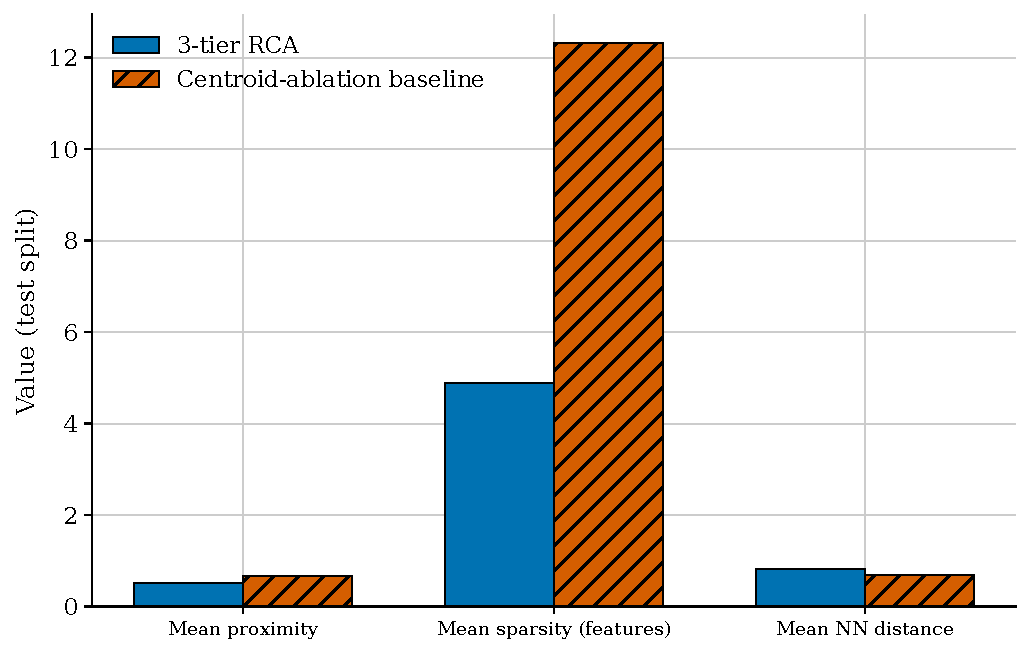
\includegraphics[width=0.75\linewidth]{fig_ch4_method_comparison_metrics.pdf}
\caption{Proximity, sparsity and nearest-neighbour distance for both methods, test split.}
\label{fig:methods}\end{figure}

\subsection{The gap is tunable}\label{sec:sweep}

\begin{table}[htbp]
\centering
\caption{Acceptance-threshold sweep, test split (iteration budget 150, $n = 147$ per row).}
\label{tab:sweep}
\small
\begin{tabular}{@{}cccccc@{}}
\toprule
$\theta$ & \textbf{Tier 1} & \textbf{Tier 2} & \textbf{Tier 3} & \textbf{Resolution} & \textbf{Confirmation} \\
\midrule
0.55 & 140 & 0  & 0   & 95.24\% & 6.43\% (9/140) \\
0.65 & 140 & 0  & 2   & 95.24\% & 9.29\% \\
0.75 & 89  & 21 & 33  & 74.83\% & 21.82\% \\
0.85 & 21  & 24 & 98  & 30.61\% & 44.44\% \\
0.95 & 1   & 6  & 137 & 4.76\%  & 85.71\% (6/7) \\
\bottomrule
\end{tabular}
\end{table}

\begin{table}[htbp]
\centering
\caption{Iteration-budget sweep, test split ($\theta = 0.55$).}
\label{tab:budget}
\small
\begin{tabular}{@{}ccc@{}}
\toprule
\textbf{Budget} & \textbf{Resolution} & \textbf{Confirmation} \\
\midrule
10  & 61.22\% & 13.33\% \\
25  & 95.24\% & 7.14\% \\
50  & 95.24\% & 6.43\% \\
150 & 95.24\% & 6.43\% \\
\bottomrule
\end{tabular}
\end{table}

Resolution falls monotonically from 95.24\% to 4.76\%; confirmation rises monotonically from 6.43\% to 85.71\%. A structurally different hyperparameter moves both in the same coupled direction. \textbf{Two knobs, one frontier} --- which is what distinguishes the finding from a badly chosen setting.

Runtime rises steeply with $\theta$, from 71~s to 1{,}084~s on test, because a stricter criterion forces more iterations and more frequent recourse to Tier 2. The cost of demanding a more confident counterfactual is paid in compute as well as in coverage.

Counts at the strict end are small and are reported as counts, not percentages alone: 85.71\% rests on 6 of 7 resolved cases, and the corresponding validation figure of 100\% on 4 of 4. These points establish the direction of the relationship, not a precise endpoint.

\begin{figure}[htbp]\centering
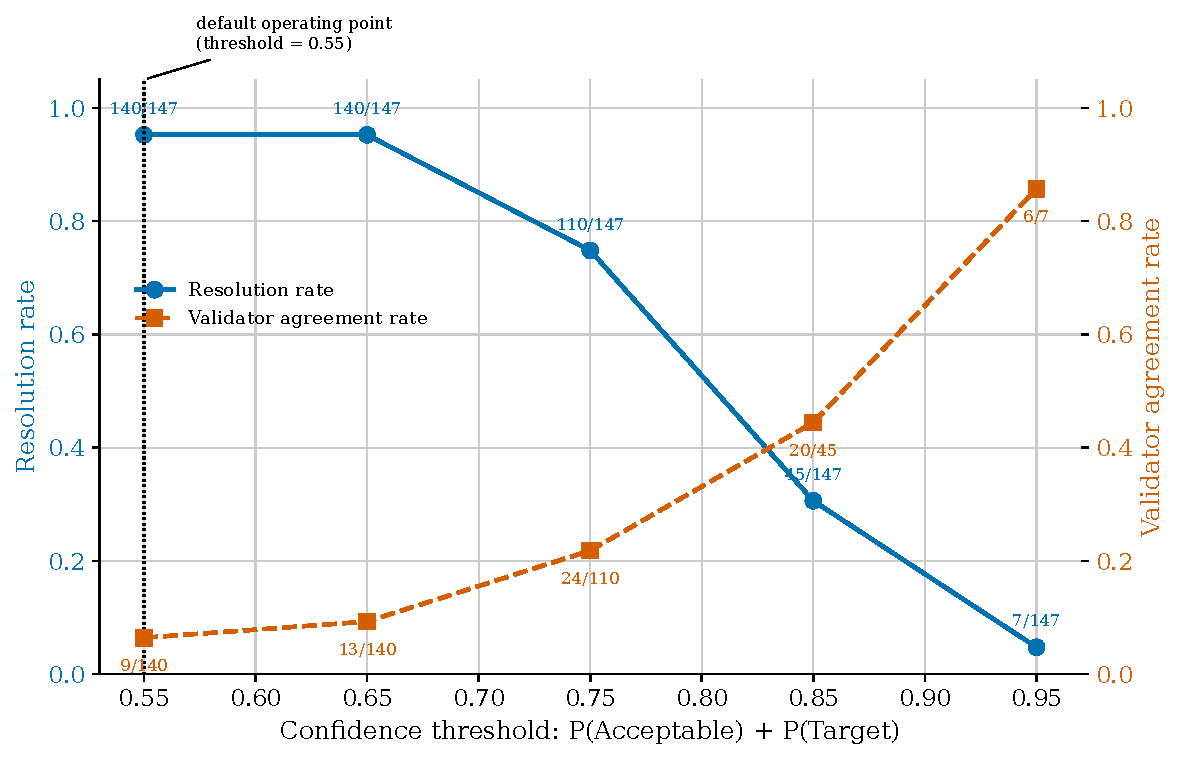
\includegraphics[width=0.85\linewidth]{fig_ch4_tradeoff_resolution_validator.pdf}
\caption{Central result. Resolution rate and independent-verifier confirmation rate as a function of the acceptance threshold, test split. Raw counts are annotated at every marker; the default operating point is marked.}
\label{fig:frontier}\end{figure}

\begin{figure}[htbp]\centering
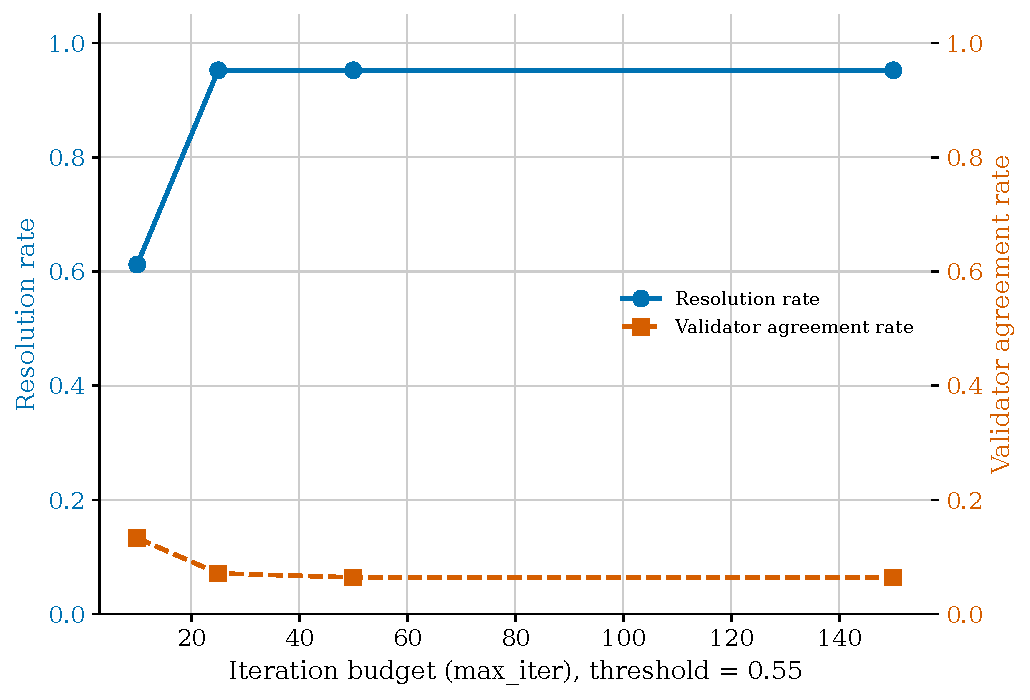
\includegraphics[width=0.75\linewidth]{fig_ch4_tradeoff_maxiter.pdf}
\caption{The same trade-off as a function of the search's iteration budget, $\theta = 0.55$, test split.}
\label{fig:budget}\end{figure}

% ------------------------------------------------------------
\section{Discussion}

\subsection{The mechanism}

A search terminating at $s(\mathbf{x}') \geq 0.55$ produces instances just inside the champion's decision boundary. Two models fitted to the same data agree strongly where the data is dense and classes well separated, and disagree in the margin --- that is what distinguishes one fitted boundary from another. A procedure designed to stop at the boundary is, by construction, a procedure for finding the points where models disagree. Raising $\theta$ pushes the endpoint into the region where both are confident, which is why confirmation rises. Truncating the budget acts through a different route with the same effect: only cycles already near the conforming region resolve, and those endpoints sit further from the margin.

Where the champion's geometry reflects a genuine process regularity, a second model trained on the same data should tend to agree. Where it reflects the particular arrangement of the training sample --- the specific placement of axis-aligned splits a random forest happens to have learned --- a model with a fundamentally different inductive bias has no reason to agree, and mostly does not.

\textbf{An additional mechanism specific to process data.} Several heavily attributed parameters --- cycle time, plasticizing time, torque peaks, clamping-force peak --- are measured outcomes rather than setpoints. Tier 1 moves its five selected parameters \emph{independently}, each in its LIME-indicated direction. A recipe that reduces filling time while increasing plasticizing time and cycle time specifies a combination of \emph{measured outcomes} that may be jointly unreachable, because no setting of the machine's actual controls produces exactly that triple. This is Karimi et al.'s objection in moving from explanation to intervention~\cite{karimi2021}: with causal dependencies among features, setting a feature to its counterfactual value does not produce the counterfactual world. Clipping guarantees each parameter individually lies within its observed range; it cannot guarantee the \emph{combination} is one the process could produce. The nearest-neighbour figure quantifies that residual, and 6.43\% is what it costs. A second model trained on real cycles has only ever seen jointly reachable combinations.

\subsection{The sparsity--validity tension}

Sparse recipes are what operators can execute. But sparsity confines the search to a low-dimensional subspace, and reaching the conforming region within it requires travelling further along each retained axis --- producing an endpoint further from the observed conforming manifold, exactly the property associated with lower confirmation. Our data show both sides: 4.88 parameters at nearest-neighbour distance 0.829 and 6.43\% confirmation, against 12.32 parameters at 0.686 and 10.00\%. A system optimising only for actionability will degrade validity with nothing in its report reflecting the fact.

\subsection{Choosing an operating point}

The frontier makes the operating point a design decision requiring justification. A deployment applying recommendations automatically needs high confirmation and belongs near $\theta = 0.85$, accepting recommendations for roughly 31\% of defective cycles and escalating the rest. A deployment using recommendations as triage hints for an engineer exercising judgement can sit lower, since the cost of a poor suggestion is attention rather than scrap.

What is not defensible is operating at $\theta = 0.55$, reporting 95.24\%, and remaining silent about the frontier.

\textbf{Counterfactual recipes should be presented to operators as hypotheses for evaluation, not as verified corrective actions.} That framing is accurate to what the evidence supports and is compatible with the operator's own process knowledge, which the system does not have.

\subsection{A validation protocol for prescriptive systems}

The three-level hierarchy of validation independence --- distributional checks, independent-model verification, and process verification --- and what each does and does not establish, is developed at length elsewhere~\cite{alqawasema2026a}; we summarise only what bears directly on this paper's application of it.

This paper operates at \textbf{Level 2}: a second model of a different family, trained on the same data with a different seed and taking no part in generation, is queried once per recommendation, and agreement is reported over the \textbf{full} evaluation population rather than selected cases. Cost here was one MLP fit and 140 predictions. Its limitation is structural, not incidental: both models share the data's biases, so agreement bounds the risk of a model-specific artefact but cannot exclude a shared one. \textbf{Level 1} (a nearest-neighbour or connectedness check~\cite{keane2021,laugel2019}, negligible cost) is weaker and was not relied on as the primary evidence here, though the nearest-neighbour distance reported in Section~\ref{sec:circ} serves that role diagnostically. \textbf{Level 3} --- enacting recommendations on the machine and measuring the resulting parts, stratified across confirmed and unconfirmed groups --- is the only definitive test and was not performed in this study; it is the natural next step, and without it a Level 2 verdict remains a proxy of unknown fidelity.

\subsection{Limitations}

\textbf{Construct validity.} The construct of interest is whether a recommended adjustment would move the part into the conforming band on a real machine. The measure used is whether a second learned model classifies the vector as conforming. These are not the same thing, and everything in Section~\ref{sec:circ} should be read as measuring the proxy.

\textbf{No process verification.} The strongest claim supported is model-level agreement. No recommended setting was applied to a machine and no resulting part measured.

\textbf{The paired test is underpowered.} McNemar's exact test ran on 9 discordant pairs. The non-significant $p = 0.180$ is weak evidence of equivalence and is not treated as more. The generalisation to a method class rests on this test \emph{plus} the structural argument about what the two methods share, and the structural argument is doing much of the work.

\textbf{Small counts at the sweep extremes.} 85.71\% at $\theta = 0.95$ rests on 7 resolved cases; the validation figure of 100\% on 4.

\textbf{The plausibility metric is structurally biased.} Nearest-neighbour distance rewards methods moving toward the conforming data mass. The ablation does that by construction, so its better score partly measures alignment between its objective and the metric's definition. Stated in advance and again at reporting, but a construct-validity limitation of that comparison.

\textbf{Resolution rate mixes two quantities}, as noted above. \textbf{The verifier flag carries two meanings} --- true both for a confirmed counterfactual and for a Tier 0 cycle the engine declined to modify --- which is why the contingency row totals exceed the confirmed counts by exactly seven, without affecting the test.

\textbf{Single dataset, single product, adopted hyperparameters.} All results derive from one dataset, one product, one machine configuration, with a champion adopted from~\cite{polenta2022} rather than tuned. Whether the frontier's shape generalises is unknown.

% ------------------------------------------------------------
\section{Conclusions}

We measured the difference between what a counterfactual root-cause analysis engine reports about itself and what an independently trained model confirms. On held-out injection molding data the engine resolves 95.24\% of non-conforming cycles; the verifier confirms 6.43\% of those resolutions. The gap is 88.81 percentage points, across the full evaluation population.

The gap does not belong to the explanation layer: an ablation discarding SHAP selection and LIME guidance reproduces it, with the difference indistinguishable from chance. It belongs to the acceptance criterion the two methods share. Sweeping that criterion from 0.55 to 0.95 moves resolution from 95.24\% to 4.76\% and confirmation from 6.43\% to 85.71\%, and sweeping the search's iteration budget moves both the same way. Resolution and confirmation are not two performance figures but two readings of one dial.

The distributional evidence identifies the mechanism: the average counterfactual sits 0.829 scaled units from the nearest real conforming cycle. The recipes land where the model labels conformance, not where conformance has been observed.

The recommendation is small and cheap. Prescriptive quality systems should report independent verification alongside self-measured resolution, and state the acceptance threshold at which both were obtained. It costs one model fit on data already in hand. It does not establish that recommendations are physically correct --- only a machine and a measurement do that --- but it converts a self-certifying claim into one that can fail.

% ------------------------------------------------------------
\section*{Back Matter}

\noindent\textbf{Author Contributions:} \TODO{CRediT statement}\\
\textbf{Funding:} \TODO{funding statement}\\
\textbf{Institutional Review Board Statement:} Not applicable.\\
\textbf{Informed Consent Statement:} Not applicable.\\
\textbf{Data Availability Statement:} The dataset analysed in this study was released by Polenta et al.~\cite{polenta2022} and is publicly available. All source code, model configurations, evaluation scripts and result artefacts supporting this work are available at \url{https://github.com/obadaqw/Thesis_Industrial_AI_V2}. \TODO{tag a release and cite the commit hash}\\
\textbf{Conflicts of Interest:} The authors declare no conflict of interest.\\
\textbf{Use of Generative AI:} \TODO{Required by MDPI. Must be consistent with Appendix G of the associated thesis.}

% ------------------------------------------------------------
\begin{thebibliography}{99}
\footnotesize

\bibitem{polenta2022} A. Polenta, S. Tomassini, N. Falcionelli, P. Contardo, A. F. Dragoni, and P. Sernani, ``A comparison of machine learning techniques for the quality classification of molded products,'' \emph{Information}, vol. 13, no. 6, art. 272, Jun. 2022, doi: 10.3390/info13060272.

\bibitem{ribeiroB2005} B. Ribeiro, ``Support vector machines for quality monitoring in a plastic injection molding process,'' \emph{IEEE Trans. Syst., Man, Cybern. C, Appl. Rev.}, vol. 35, no. 3, pp. 401--410, Aug. 2005, doi: 10.1109/TSMCC.2004.843228.

\bibitem{parizs2022} R. D. P\'{a}rizs, D. T\"{o}r\"{o}k, T. Ageyeva, and J. G. Kov\'{a}cs, ``Machine learning in injection molding: An Industry 4.0 method of quality prediction,'' \emph{Sensors}, vol. 22, no. 7, art. 2704, Apr. 2022, doi: 10.3390/s22072704.

\bibitem{ogorodnyk2019} O. Ogorodnyk, O. V. Lyngstad, M. Larsen, K. Wang, and K. Martinsen, ``Application of machine learning methods for prediction of parts quality in thermoplastics injection molding,'' in \emph{Advanced Manufacturing and Automation VIII}. Singapore: Springer, 2019, pp. 237--244, doi: 10.1007/978-981-13-2375-1\_30.

\bibitem{muller2022} D. M\"{u}ller, M. M\"{a}rz, S. Scheele, and U. Schmid, ``An interactive explanatory AI system for industrial quality control,'' in \emph{Proc. AAAI Conf. Artificial Intelligence}, vol. 36, no. 11, 2022, pp. 12580--12586, doi: 10.1609/aaai.v36i11.21530.

\bibitem{ribeiro2016} M. T. Ribeiro, S. Singh, and C. Guestrin, ```Why should I trust you?': Explaining the predictions of any classifier,'' in \emph{Proc. 22nd ACM SIGKDD Int. Conf. Knowledge Discovery and Data Mining}, 2016, pp. 1135--1144, doi: 10.1145/2939672.2939778.

\bibitem{wachter2018} S. Wachter, B. Mittelstadt, and C. Russell, ``Counterfactual explanations without opening the black box: Automated decisions and the GDPR,'' \emph{Harvard J. Law Technol.}, vol. 31, no. 2, pp. 841--887, 2018.

\bibitem{mothilal2020} R. K. Mothilal, A. Sharma, and C. Tan, ``Explaining machine learning classifiers through diverse counterfactual explanations,'' in \emph{Proc. 2020 Conf. Fairness, Accountability, and Transparency (FAT* '20)}, 2020, pp. 607--617, doi: 10.1145/3351095.3372850.

\bibitem{verma2024} S. Verma, V. Boonsanong, M. Hoang, K. Hines, J. Dickerson, and C. Shah, ``Counterfactual explanations and algorithmic recourses for machine learning: A review,'' \emph{ACM Comput. Surv.}, vol. 56, no. 12, art. 312, pp. 1--42, Dec. 2024, doi: 10.1145/3677119.

\bibitem{guidotti2024} R. Guidotti, ``Counterfactual explanations and how to find them: Literature review and benchmarking,'' \emph{Data Min. Knowl. Discov.}, vol. 38, no. 5, pp. 2770--2824, 2024, doi: 10.1007/s10618-022-00831-6.

\bibitem{poyiadzi2020} R. Poyiadzi, K. Sokol, R. Santos-Rodriguez, T. De Bie, and P. Flach, ``FACE: Feasible and actionable counterfactual explanations,'' in \emph{Proc. AAAI/ACM Conf. AI, Ethics, and Society (AIES)}, 2020, pp. 344--350, doi: 10.1145/3375627.3375850.

\bibitem{vanlooveren2021} A. Van Looveren and J. Klaise, ``Interpretable counterfactual explanations guided by prototypes,'' in \emph{Machine Learning and Knowledge Discovery in Databases (ECML PKDD)}. Cham, Switzerland: Springer, 2021, pp. 650--665, doi: 10.1007/978-3-030-86520-7\_40.

\bibitem{ustun2019} B. Ustun, A. Spangher, and Y. Liu, ``Actionable recourse in linear classification,'' in \emph{Proc. Conf. Fairness, Accountability, and Transparency (FAT* '19)}, 2019, pp. 10--19, doi: 10.1145/3287560.3287566.

\bibitem{karimi2021} A.-H. Karimi, B. Sch\"{o}lkopf, and I. Valera, ``Algorithmic recourse: From counterfactual explanations to interventions,'' in \emph{Proc. ACM Conf. Fairness, Accountability, and Transparency (FAccT)}, 2021, pp. 353--362, doi: 10.1145/3442188.3445899.

\bibitem{keane2021} M. T. Keane, E. M. Kenny, E. Delaney, and B. Smyth, ``If only we had better counterfactual explanations: Five key deficits to rectify in the evaluation of counterfactual XAI techniques,'' in \emph{Proc. 30th Int. Joint Conf. Artificial Intelligence (IJCAI-21)}, Survey Track, 2021, pp. 4466--4474, doi: 10.24963/ijcai.2021/609.

\bibitem{laugel2019} T. Laugel, M.-J. Lesot, C. Marsala, X. Renard, and M. Detyniecki, ``The dangers of post-hoc interpretability: Unjustified counterfactual explanations,'' in \emph{Proc. 28th Int. Joint Conf. Artificial Intelligence (IJCAI-19)}, 2019, pp. 2801--2807, doi: 10.24963/ijcai.2019/388.

\bibitem{nauta2023} M. Nauta, J. Trienes, S. Pathak, E. Nguyen, M. Peters, Y. Schmitt, J. Schl\"{o}tterer, M. van Keulen, and C. Seifert, ``From anecdotal evidence to quantitative evaluation methods: A systematic review on evaluating explainable AI,'' \emph{ACM Comput. Surv.}, vol. 55, no. 13s, art. 295, pp. 1--42, Jul. 2023, doi: 10.1145/3583558.

\bibitem{alvarezmelis2018} D. Alvarez-Melis and T. S. Jaakkola, ``On the robustness of interpretability methods,'' arXiv:1806.08049, Jun. 2018.

\bibitem{slack2020} D. Slack, S. Hilgard, E. Jia, S. Singh, and H. Lakkaraju, ``Fooling LIME and SHAP: Adversarial attacks on post hoc explanation methods,'' in \emph{Proc. AAAI/ACM Conf. AI, Ethics, and Society (AIES)}, 2020, pp. 180--186, doi: 10.1145/3375627.3375830.

\bibitem{krishna2022} S. Krishna, T. Han, A. Gu, J. Pombra, S. Jabbari, S. Wu, and H. Lakkaraju, ``The disagreement problem in explainable machine learning: A practitioner's perspective,'' arXiv:2202.01602, Feb. 2022.

\bibitem{adebayo2018} J. Adebayo, J. Gilmer, M. Muelly, I. Goodfellow, M. Hardt, and B. Kim, ``Sanity checks for saliency maps,'' in \emph{Advances in Neural Information Processing Systems (NeurIPS)}, vol. 31, 2018, pp. 9505--9515.

\bibitem{doshivelez2017} F. Doshi-Velez and B. Kim, ``Towards a rigorous science of interpretable machine learning,'' arXiv:1702.08608, Mar. 2017.

\bibitem{breiman2001} L. Breiman, ``Random forests,'' \emph{Mach. Learn.}, vol. 45, no. 1, pp. 5--32, Oct. 2001, doi: 10.1023/A:1010933404324.

\bibitem{geurts2006} P. Geurts, D. Ernst, and L. Wehenkel, ``Extremely randomized trees,'' \emph{Mach. Learn.}, vol. 63, no. 1, pp. 3--42, Apr. 2006, doi: 10.1007/s10994-006-6226-1.

\bibitem{pedregosa2011} F. Pedregosa \emph{et al.}, ``Scikit-learn: Machine learning in Python,'' \emph{J. Mach. Learn. Res.}, vol. 12, pp. 2825--2830, 2011.

\bibitem{cawley2010} G. C. Cawley and N. L. C. Talbot, ``On over-fitting in model selection and subsequent selection bias in performance evaluation,'' \emph{J. Mach. Learn. Res.}, vol. 11, pp. 2079--2107, 2010.

\bibitem{page1954} E. S. Page, ``Continuous inspection schemes,'' \emph{Biometrika}, vol. 41, no. 1--2, pp. 100--115, Jun. 1954, doi: 10.1093/biomet/41.1-2.100.

\bibitem{lundberg2017} S. M. Lundberg and S.-I. Lee, ``A unified approach to interpreting model predictions,'' in \emph{Advances in Neural Information Processing Systems (NeurIPS)}, vol. 30, 2017, pp. 4765--4774.

\bibitem{rudin2019} C. Rudin, ``Stop explaining black box machine learning models for high stakes decisions and use interpretable models instead,'' \emph{Nat. Mach. Intell.}, vol. 1, no. 5, pp. 206--215, May 2019, doi: 10.1038/s42256-019-0048-x.

\bibitem{mcnemar1947} Q. McNemar, ``Note on the sampling error of the difference between correlated proportions or percentages,'' \emph{Psychometrika}, vol. 12, no. 2, pp. 153--157, Jun. 1947, doi: 10.1007/BF02295996.

\bibitem{alqawasema2026a} O. AlQawasema, ``How do we know a counterfactual is right? A critical review of validation practice for prescriptive explainable AI in manufacturing quality control,'' \TODO{Preprints.org, 2026. Add DOI once posted (see README\_papers.md).}

\end{thebibliography}

\end{document}
